\label{sec:results}

%
% RESULTS TODO
%
% need to motivate optimization workflow and plans
% current ideas not bad, need more
%
%

The computer simulations in the proposed study are intended to discover
the optimal solar vortex system configuration for a range of scenarios
and system sizes. This section contains discussions of the preliminary
simulation results to motivate that the existing simulation capability
is sufficiently well developed and understood to permit an efficient
exploration of the SoV configuration space. 
This section begins with a discussion of the structure of solutions from
a representative case with no ambient winds, the ``thermal only''
scenario. Next, a case with strong ambient horizontal winds (``Wind'')
is discussed. Finally, the results from a series of runs are shown to
demonstrate a heuristic by which incremental optimization of the system
configuration will be conducted\todo{fix this sentence}.

%The results of these optimized configurations will be used as input
%for the design of a prototype to be tested in Mesa, Arizona this
%summer. 

% \todo{add photo}
  % \begin{figure}[!htb]
  %  \begin{center}
  %   \includegraphics[width = 12 cm]{figs/sov_field}
  %   \caption{A photo of the field configuration, during the June 2015
  %   Field Test.}
  %   \label{fig:field_real}
  %  \end{center}
  % \end{figure}

\section{Thermal Only}

While ambient winds in the field impact system performance, it is
also illuminating to consider an idealized scenario with natural convection
driven only by thermal instabilities. Simulations of this baseline,
thermal-only flow are intended to ensure the SoV apparatus to form a
strong thermal plume even in the absence of wind. 

In this section a representative case of an optimized thermal-only SoV
configuration is presented. This is a simple curved vane configuration with
two-tiers with ground temperature of 335 Kelvin and a freestream
temperature of 313 Kelvin. There is no ambient velocity and the boundary
conditions are as described in Chapter \ref{sec:bc}. 

The two tiers of vanes used for these cases are drawn in Figures
\ref{fig:thermal_vane_bottom} and \ref{fig:thermal_vane_top}.
 Note that in the
configuration, the vanes are 
aligned radially at the largest radius, and then increasingly curve
towards azimuthal at smaller radius. Note that these are representative
curves of the body forcing field, and do not actually represent vane
surfaces. The vanes are represented as in Chapter \ref{subsec:vane}. 
These images are created by tracing the path a particle follows through
the forcing field. The region of forcing is between $\{0.3-0.9\}$ meters
for the bottom tier, and $\{0.6-0.9\}$ meters for the top tier. Overall,
the system is 1.1 meters tall, with the short first tier only standing
0.132 meters high. The top and bottom tiers have final angles of
$70^{\circ}$ and $85^{\circ}$, respectively. No cone is used in this
case. 

\begin{figure}[htb]
\centering
\begin{minipage}{0.45\textwidth}
\centering
 \includegraphics[width=.8\linewidth]{figs/bottom_thermal_only}
 \caption{Horizontal drawings of the curvature functions for the bottom tier
 vanes. The max angle is $85^{\circ}$, or $5^{\circ}$ less than azimuthal.}
 \label{fig:thermal_vane_bottom}  
\end{minipage}\hfill
\begin{minipage}{0.45\textwidth}
\centering
\includegraphics[width =0.8\textwidth]{figs/top_thermal_only}
\caption{Horizontal drawings of the curvature functions for the top tier
 vanes. The max angle is $70^{\circ}$, or $20^{\circ}$ less than
 azimuthal.} 
 \label{fig:thermal_vane_top}  
\end{minipage}
\end{figure}

\begin{figure}[htb]
\centering
\begin{minipage}{0.45\textwidth}
\centering
 \includegraphics[width=.8\linewidth]{figs/3d}
 \caption{Isocountours of the inner thermal core
  visible through semi-transparent contour around azimuthal velocity,
  colored by vertical velocity. This shows that the thermal core creates
 an upward flow, which entrains and rotations fluid around it. An
 outline of the region of virtual vanes has been drawn.}
 \label{fig:thermal}  
\end{minipage}\hfill
\begin{minipage}{0.45\textwidth}
\centering
\includegraphics[width =0.8\textwidth]{figs/entrainment}
\caption{Fluid entrainment around the apparatus. This was drawn by
 seeding particles into the averaged flowfield and then advancing them
 using an RK4 time integrator. An outline of the
  virtual vanes are drawn to show the region of forcing.}
 \label{fig:entrain}  
\end{minipage}
\end{figure}


% \begin{figure}[htb]

%  \begin{subfigure}{.55\textwidth}
%   \centering
%   \includegraphics[width =0.7\textwidth]{figs/3d}
%   \caption{Isocountours of the inner thermal core
%   visible through semi-transparent contour around azimuthal velocity,
%   colored by vertical velocity. An outline of the region of virtual
%   vanes has been drawn.}
%   \label{fig:thermal}  
%  \end{subfigure}%
%  \begin{subfigure}{.4\textwidth}
%   \centering
%   \includegraphics[width =0.8\textwidth]{figs/entrainment}%
%   \caption{Fluid entrainment around the apparatus. An outline of the
%   virtual vanes are drawn to show the region of forcing.} 
%   \label{fig:entrain}  
%  \end{subfigure}%
% \end{figure}

The results shown are the averages of fifty snapshots of the solution 
taken over the course of ten minutes. In general, the averaging times
are selected to be approximately 20 to 30 wash-out times, where a
wash-out is defined as the time required for a particle at the base of
the apparatus to flow out through the top boundary. The kinetic energy flux
through the top of the vanes for this case is about 53 watts. The solution
demonstrates several features characteristic of naturally occurring dust
devils. Figure \ref{fig:thermal} shows a temperature isocontour set at
threshold of 3 Celsius higher than the ambient fluid temperature. This
value was selected because it was noted by
Sinclair\cite{Sinclair1969} as characteristic of the thermal core
temperature above the ambient temperature observed in dust devils. The
image depicts a tight, coherent thermal plume roughly the same size as
the inner diameter of the lower vanes. As anticipated, this hot flow is
acting like a chimney, generating a large vertical velocity which in
turn entrains air from the outside.  

An image of the entrainment is shown in Figure\ref{fig:entrain}. The
image was created by tracking particles as they 
convect through the device. Tracer particles were seeded into the
averaged flowfield and then advancing through 
the field using an RK4 time integrator. 
\todo{define how this is actually performed, mathematically}
 There is clearly a tight inner vortex with significant azimuthal
 velocity and a broader region of entraining fluid through the
 upper tier of vanes.   

% \begin{figure}[htb]

%  \begin{subfigure}{.5\textwidth}
%   \centering
%   \includegraphics[width=.75\linewidth]{figs/vt}
%   \caption{Azimuthal Velocity}
%   \label{fig:vt-to}
%  \end{subfigure}%
%  \begin{subfigure}{.5\textwidth}
%   \centering
%   \includegraphics[width=.8\linewidth]{figs/vz}
%   \caption{Vertical Velocity}
%   \label{fig:vz-to}
%  \end{subfigure}%


%  \begin{subfigure}{.5\textwidth}
%   \centering
%   \includegraphics[width=.85\linewidth]{figs/t}
%   \caption{Temperature}
%   \label{fig:t-to}
%  \end{subfigure}%
%  \begin{subfigure}{.5\textwidth}
%   \centering
%   \includegraphics[width=.75\linewidth]{figs/p}
%   \caption{Pressure}
%   \label{fig:p-to}
%  \end{subfigure}%

%  \caption{Time averaged vertical slices through the center of the device
%  for the thermal-only cases. Black lines indicate the location of the
%  vanes. A strong thermal plume is visible at the center of the device,
%  which drives a vertical velocity. The fluid flow is entrained by this
%  vertical movement and pulled radially into the center while being
%  turned by the turning vanes. Notice also the low pressure ``eye'' at
%  the center of the flow,and the modest downward flow in the
%  center of the vertical velocity, consistent with Figure \ref{fig:cartoon}.}
%  \label{fig:to-vert}
% \end{figure}

%
%
%
Figure \ref{fig:to-vert} depicts several vertical slices through the SoV
for various state variables. One can see that there is a tight core
vortex with azimuthal and vertical velocities of several meters per
second. The tight vortex region coincides with a high temperature, low
pressure core region. The rapidly rotating air near the center induces
a low pressure core, as observed in real dust devils.
On the vertical velocity plot, a small downward flow region has formed in
the middle of the vortex, consistent with the sketch in Figure
\ref{fig:cartoon}.  

\begin{figure}[htb]

 \centering
  \includegraphics[width=.32\linewidth]{figs/vt_hor}
 %\caption{Azimuthal Velocity}
 % \label{fig:vt-to}
 \hfill
  \includegraphics[width=.32\linewidth]{figs/vz_hor}
 % \caption{Vertical Velocity}
 % \label{fig:vz-to}
 \hfill
  \includegraphics[width=.32\linewidth]{figs/t_hor}
 % \caption{Temperature}
 % \label{fig:t-to}
 \caption{Time averaged horizontal slices taken at the height of the
 second tier of vanes for the thermal-only cases. These images show a
 clear thermal plume driving a strong vertical velocity. Notice also the
 low downward velocity ``eye of the storm'' in (a). In contrast to the
 wind cases, the vortex is well-anchored in the center of the apparatus. }
 \label{fig:to-hor}
\end{figure}

Figure \ref{fig:to-hor}, depicts several horizontal slices
through the SoV for the same state variables. It can be seen that the
large velocities are highly localized to a region just inside the
vanes. Likewise, the entrainment of fluid is limited to a region
immediately surrounding the vanes. 
%
% conclusion of thermal only
%
Finally, the thermal plume is relatively
narrow compared to the diameter of the device. It is desirable to
broaden the thermal plume, as this would create a larger vertical
momentum flux and consequentally a larger kinetic energy flux. 
%% This will presumably
%% entrain more surrounding fluid, driving it through the vanes and
%% imparting kinetic energy to the flow. The kinetic energy grows as the
%% square of the radius, so any broadening of the vortex core can greatly
%% enhance the kinetic energy flux. 
The diameter of the thermal core is therefore a critical flow
characteristic in the thermal-only conditions. However, a means of
setting the thermal plume's thickness is not presently 
known. Regardless, these slices lend credibilty to the 
notion that our turning vane configuration is generating something with
visible parallels to a naturally occurring dust devil.   

\section{Wind}

The wind case is for a 5 m/s ambient wind with a ground temperature of
335 Kelvin and freestream temperature of 313 Kelvin. There is no ambient
velocity and the boundary conditions are as described in Chapter
\ref{sec:bc}. The vanes are drawn in Figures \ref{fig:wind_bottom} and
\ref{fig:wind_top}. These images show the straight vane case, and
a cone that sits on top of the second tier of vanes. 
As in the previous section, these images are representative
curves of the body forcing field, and do not actually represent vane
surfaces. The vanes are represented as in Chapter \ref{subsec:vane}. 
These images are created by tracing the path a particle follows through
the forcing field. The region of forcing is between $\{0.96-3.4\}$ meters
for the bottom tier, and $\{1.5-3.4\}$ meters for the top tier. Overall,
the system is three meters tall, with the short first tier only standing
0.3 meters high. The top and bottom tiers have final angles of
$70^{\circ}$ and $80^{\circ}$, respectively. 

\begin{figure}[htb]
\centering
\begin{minipage}{0.45\textwidth}
\centering
 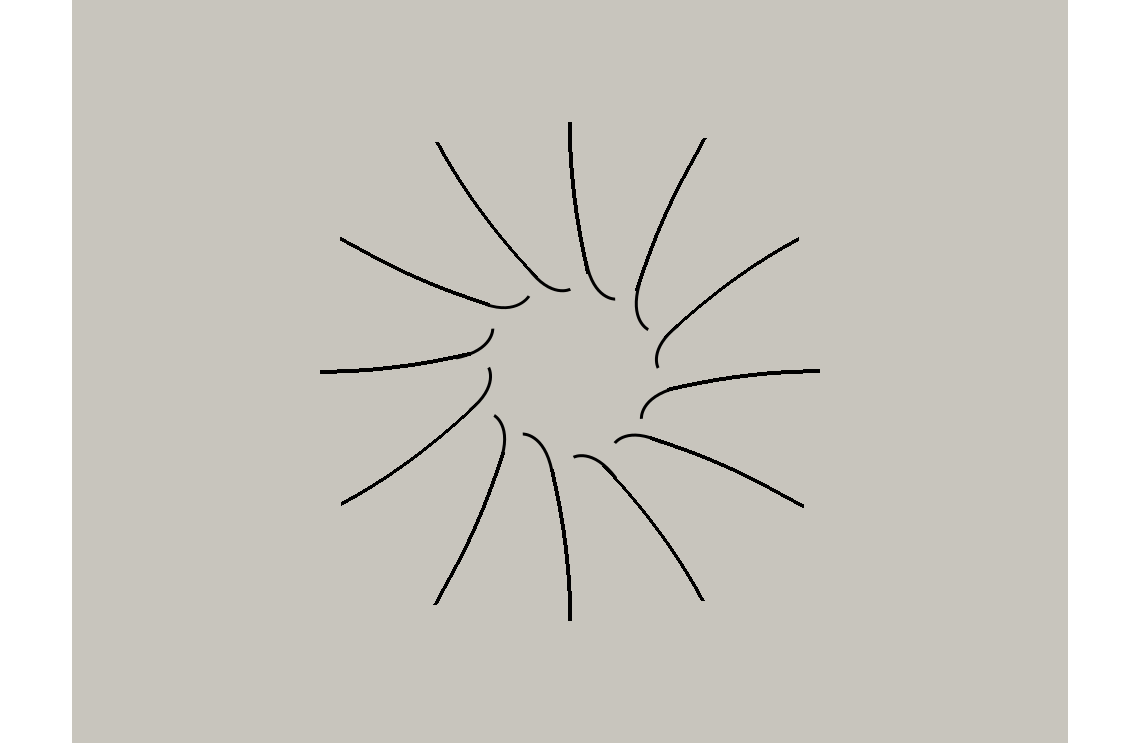
\includegraphics[width=.8\linewidth]{figs/wind_bottom}
 \caption{Horizontal drawings of the bottom tier vanes. These are curved 
 vanes with a final angle of $80^{\circ}$.}
 \label{fig:wind_bottom}  
\end{minipage}\hfill
\begin{minipage}{0.45\textwidth}
\centering
\includegraphics[width =0.8\textwidth]{figs/wind_top}
\caption{Horizontal drawings of the top tier vanes. These are straight
 angle vanes set at $70^{\circ}$.} 
 \label{fig:wind_top}  
\end{minipage}
\end{figure}


%
% horizontal slices
%
\begin{figure}[htb]

  \centering
  \includegraphics[width=.47\linewidth]{figs/wind_u}
 %\caption{Streamwise}
 % \label{fig:vt-wind}
 \hfill
  \includegraphics[width=.47\linewidth]{figs/wind_w}
 %\caption{Vertical Velocity}
 % \label{fig:vz-wind}
 \\
  \centering
  \includegraphics[width=.47\linewidth]{figs/wind_t}
 \hfill
  \includegraphics[width=.47\linewidth]{figs/wind_p}
  %\label{fig:p-wind}
 \caption{Time averaged horizontal slices taken at the height of the
 vanes for the wind cases. The streamwise velocity shows a large
 penetration in the region where the vanes are not blocking, and in the
 other regions the flow is blocked and flows around. The vertical
 velocity is disorganized and does not show the ``two cell'' structure
 as in the thermal-only cases.  Note that an
 off-center thermal plume is visible, as well.  } 
 \label{fig:wind-hor}
\end{figure}


Horizontal slices of the azimuthal and vertical velocities, and the 
temperature and pressure fields are shown in Figure
\ref{fig:vz-wind-vert}. The freestream velocity is traveling from left
to right at 5$ m/s$, which was set based on ambient velocity
measurements made by  the experimental team from the field. While the
structure is undoubtedly different than the thermal-only cases shown
previously, we can nevertheless see that a thermal plume is forming
along with a rotating velocity structure. In general the wind cases are
more disorganized, with less obviously visible coherent
structure. Notice however that the magnitude of velocities are several
times larger than in the thermal-only cases, and the kinetic energy
flux through the vanes is also significantly higher.  

%
% vertical
%

% \begin{figure}[htb]

%  \begin{subfigure}{.5\textwidth}
%   \centering
%   \includegraphics[width=.75\linewidth]{figs/wind_u_vertical}
%   \caption{Streamwise}
%   \label{fig:vt-wind-vert}
%  \end{subfigure}%
%  \begin{subfigure}{.5\textwidth}
%   \centering
%   \includegraphics[width=.8\linewidth]{figs/wind_w_vertical}
%   \caption{Vertical Velocity}
%   \label{fig:vz-wind-vert}
%  \end{subfigure}%


%  \begin{subfigure}{.5\textwidth}
%   \centering
%   \includegraphics[width=.85\linewidth]{figs/wind_t_vertical}
%   \caption{Temperature}
%   \label{fig:t-wind-vert}
%  \end{subfigure}%
%  \begin{subfigure}{.5\textwidth}
%   \centering
%   \includegraphics[width=.75\linewidth]{figs/wind_p_vertical}
%   \caption{Pressure}
%   \label{fig:p-wind-vert}
%  \end{subfigure}%

%  \caption{Time averaged vertical slices from the center of the device
%  for the wind cases. A great deal of flow is radially entrained by the
%  first tier of vanes, consistent with the approach proposed in
%  Figure \ref{fig:cartoon_vanes}. 
%  Notice that while the temperature field appears to
%  be quite modest, this is due to the fact that the thermal column is not
%  well centered. The full column is quite visible in Figure
%  \ref{fig:field_real}.}  
%  \label{fig:wind-ver}
% \end{figure}

The vertical slices are shown in Figure~\ref{fig:wind-ver}. In this
case, the lower tier of vanes are where the majority of flow is 
entering the center of the apparatus, while the second tier of vanes are
blocking the ambient wind and providing protection for the vortex column. 

The thermal plume is significantly less
visible than in the thermal-only cases. While the
thermal-plume is necessarily weaker relative to the wind, some of this
is also due to the plume no longer being directly centered in the
flow. The plume is more visible using isocountors to render a
three-dimensional surface. 
To visualize the difference between the vertically varying ambient
temperature and the warmer thermal plume, we use the potential
temperature, defined as, 
\begin{equation}
  \tau(x,y,z) = T(x,y,z) -T_{\text{in}}(z) 
   \label{eqn:tau}
\end{equation}
where $T_{\text{in}}$ is the inflow temperature, described
in Chapter \ref{sec:bc}. In this way the background potential
temperature is nearly zero, and larger values represent deviations from
the base flow temperature. The isocountour of a three Kelvin is 
shown in Figure \ref{fig:field_real}. This value was selected as
it was noted as sufficient for formation of a dust devil by
Sinclair\cite{Sinclair1969}. It is clear from the image that a 
strong thermal column does exist even in the $5 m/s$ wind cases. 

%
% tiso
%
  \begin{figure}[!htb]
   \begin{center}
    \includegraphics[width = 12 cm]{figs/t_iso}
    \caption{Iso-contour of the thermal plume. Here, the isocontour is
    labelled by the potential temperature, $\tau$, as defined in
    Equation \ref{eqn:tau}. A strong thermal column has visibly formed. The
    figure is colored by the streamwise velocity, and shows the thermal
    column also has rotation.} 
    \label{fig:field_real}
   \end{center}
  \end{figure}

\section{Optimization}

In this section results from a representative optimization
in a thermal-only case are discussed, to demonstrate the optimization 
process employed so far. This is a typical mode of scientific and
engineering inquiry, where a hypothesis regarding system operation is
developed, followed by testing of the hypothesis, and further
iterations.  

This series of simulations are all runs with different system
configurations conducted in a common ambient scenario, that of the
unsteady thermal-only simulations described in Chapter \ref{sec:bc}. 

Our objective is to maximize the energy that can be 
extracted from the synthetic dust devil. As a surrogate to this
quantity, consider the kinetic energy flux through a horizontal plane
near the top of the vanes, where a turbine will ultimately be
placed. This is a surface integral\cite{landau1959fm}

%% \begin{equation}
%%  \dot E = -\oint \rho \textbf{v}(\frac{1}{2}v^2 + e) \cdot d \textbf{f}
%% \end{equation}
%% where $e$ is the internal energy. % and $d\textbf{f}$ the. 
%% For our problem, we consider an incompressible fluid flowing through a
%% flat horizontal region interior to the vanes in the x-y plane, which
%% results in, 

 \begin{equation}
 \dot E = -\frac{\rho }{2} \int V_z (V_{\theta}^2 + V_z^2 ) dA.
 \end{equation}

\begin{figure}[htb]
 \centering
 \includegraphics[width=.75\linewidth]{figs/opt_plot}
 \caption{This plot diagrams the improvements to the calculated flux for  
 each iteration of system configuration. Every iteration is labeled by
 design change.}
 \label{fig:opt_plot}
\end{figure}


% \begin{figure}[htb!]
%  \begin{subfigure}{.5\textwidth}
%   \centering
%   \includegraphics[width=.75\linewidth]{figs/before_vanes}
%   \caption{Vanes before optimization}
%  \end{subfigure}%
%  \begin{subfigure}{.5\textwidth}
%   \centering
%   \includegraphics[width=.8\linewidth]{figs/after_vanes}
%   \caption{Vanes after optimization}
%  \end{subfigure}%
%   \caption{Can we do this}
%  \label{fig:vt-wind-vert}
% \end{figure}\todo{need better figure}


%
%
% \begin{figure}[htb!]
%  \begin{subfigure}{.5\textwidth}
%   \centering
%   \includegraphics[width=.75\linewidth]{figs/before_opt}
%   \caption{Flow before optimization}
%  \end{subfigure}%
%  \begin{subfigure}{.5\textwidth}
%   \centering
%   \includegraphics[width=.8\linewidth]{figs/after_opt}
%   \caption{Flow after optimization}
%  \end{subfigure}%
%   \caption{These are vertical slices taken at the center of the vanes of
%  the vertical velocity taken before and after the numerous optimizations
%  of the turning vanes detailed in Figure \ref{fig:opt_plot}. In the
%  original figure, the flow produces a narrow plume. In the second, the
%  flow shows stronger vertical velocities in a much larger and more
%  organized vortex. The flow has also transitioned into a ``two-cell''
%  structure akin to that observed in the naturally occuring phenomena as
%  discussed in Chapter \ref{subsec:phenomena}}
%   \label{fig:opt_flow}
% \end{figure}
%

Using the kinetic energy flux as an objective, the vane geometry has
been optimized. Over approximately tens of iterations, we have
increased the kinetic energy flux by a factor of 88 relative to the
baseline. 
%Results of several of these iterations are documented in
%Figure \ref{fig:opt_plot}. 
Major adjustments to design in the the vane
shape and angles were made to obtain this improvement. Before and after
images are shown in Figure \ref{fig:vt-wind-vert}. During this
optimization the 
qualitative character of the solution changed substantially, changing
from a mild upward flow with little rotation to a strongly organized
vortex with a downward central flow and strong azimuthal
velocities. Before and after vertical slices are shown in Figure
\ref{fig:opt_flow}. Nevertheless, with a peak energy flux for the final 
iteration of less than one hundred Watts, significant further
optimization is necessary for this system to be viable for use as an 
energy production system. This naturally leads to the next section,
which is a discussion of the proposed research campaign. 

\section{The Effect of the Wind}
\label{sec:wind_impact}

% Regarding question number 2, you want to optimize the lift vector (see
% the figure below).  For the figure, pretend you are sitting to the side
% of the turbine as the blade is moving up.  We want the L vector to be as
% close to vertical as possible (in the useful torque direction that will
% pull the blade up).  In order to do that you need to optimize the
% Lift/Drag, but you also need to minimize the downwash (Utheta0 and Uz0
% vectors) as the downwash will turn the lift vector away from the useful
% torque direction.   Atkins and Liebeck show how to minimize the downwash
% at a given design condition for a given a set of optimum airfoils.  You
% can directly solve for blade twist and planform to make sure downwash is
% minimized and each airfoil is at its Max L/D, but this often gives rotor
% designs that are not robust and structurally infeasible.
% However, it will give you an idea of what the ideal blade looks like at
% different conditions and then you can work to find a more robust
% solution and add structural constraints as well.   

The   propulsor   has   been   modelled   using the actuator    disc
simplification.  Thereto,    the  propulsor  is  lumped  into  a  single
disc  with  no axial dimension.  The  effect  of  the  propulsor  is
then  obtained  by  assuming  a  uniform  pressure  difference across
the  disc,  implicitly  given by a  momentum  balance  around  the
propulsor and the thrust created  by  the  propulsor.


\section{Energy Scaling with Vortex Size}

